\documentclass{article}
\usepackage[utf8]{inputenc}
\usepackage[mmddyyyy]{datetime}
\usepackage{algorithm}
\usepackage{algpseudocode}
\usepackage{graphicx}
\usepackage{natbib}
\bibliographystyle{unsrtnat}

\title{CME 211 Software Development for Scientists and Engineers - Final Project}
\author{Leon H. Kloker}
\date{\today}

\begin{document}

\maketitle

\section{Summary}

This project revolves around solving the steady-state heat equation in 2 dimensions on a rectangular domain via central finite differences with C++. The domain has periodic boundaries in the lateral directions and Dirichlet boundaries at the top and bottom. The arising sparse linear equation system is solved iteratively with the Conjugate Gradient algorithm. The iterate solutions are written to files and can be read with a python postprocessing script in order to visualize the solution.

\section{CG solver}

In order to implement the CG solver in C++, we have to write our own library of linear algebra functions in order to perform matrix-vector or vector-vector operations. In the file \texttt{matvecops.cpp}, the following functions were implemented in order to avoid duplicate code in the CG algorithm: 
\begin{enumerate}

\item \texttt{vector\_addition} - This function adds to vectors together elementwise.

\item \texttt{vector\_subtraction} - This function subtracts two vectors from each other.

\item \texttt{scalar\_multiplication} - This function multiplies every element in a vector by the given scalar.

\item \texttt{scalar\_product} - This function calculates the scalar product of two vectors.

\item \texttt{l2\_norm} - This function calculates the L2 norm of a vector.
    
\end{enumerate}

Moreover, in \texttt{sparse.cpp}, a SparseMatrix class is implemented which comprises the following function:
\begin{enumerate}

\item \texttt{AddEntry} - This function adds a new entry to the sparse matrix.

\item \texttt{ConvertToCSR} - This function converts the matrix to CSR format.

\item \texttt{MulVec} - This function multiplies the matrix by a given vector.
    
\end{enumerate}

Finally, the CG solver method itself is implemented in \texttt{CGSolver.cpp}, where the \texttt{CGSolver} method takes a SparseMatrix, right-hand side vector, initial solution guess and a tolerance. Using the methods previously described, the implementation of the CG solver pseudo-code in algorithm \ref{code} is straightforward.

\vspace{0.5cm}
\begin{algorithm}
\caption{CG solver}\label{alg:cg}
\label{code}
\begin{algorithmic}
\State Initialize $x_0$
\State $r_0 = b - Ax_0$
\State L2normr0 = $||r_0||_2$
\State $p_0 = r_0$
\State $n = 0$
\While{$n <$ nmax}
\State $\alpha = r_n^T r_n / p_n^T A p_n$
\State $x_{n+1} = x_n + \alpha p_n$
\State $r_{n+1} = r_n - \alpha A p_n$
\State L2normr = $||r_{n+1}||_2$
\If{L2normr / L2normr0 $<$ threshold}
\State break
\EndIf
\State $\beta = r_{n+1}^T r_{n+1} / r_n^T r_n$
\State $p_{n+1} = r_{n+1} + \beta p_n$
\State $n = n + 1$
\EndWhile
\end{algorithmic}
\end{algorithm}

\section{Exemplary Usage}
Build the executable file:\\
\texttt{\$make\\
g++ -std=c++11 -Wall -Wconversion -Wextra -Wpedantic -c main.cpp\\
g++ -std=c++11 -Wall -Wconversion -Wextra -Wpedantic -c CGSolver.cpp\\
g++ -std=c++11 -Wall -Wconversion -Wextra -Wpedantic -c COO2CSR.cpp\\
g++ -std=c++11 -Wall -Wconversion -Wextra -Wpedantic -c matvecops.cpp\\
g++ -std=c++11 -Wall -Wconversion -Wextra -Wpedantic -c heat.cpp\\
g++ -std=c++11 -Wall -Wconversion -Wextra -Wpedantic -c sparse.cpp\\
g++ -O3 -std=c++11 -Wall -Wconversion -Wextra -Wpedantic main.o CGSolver.o heat.o sparse.o COO2CSR.o matvecops.o -o main}\\
\vspace{0.05cm}\\
Solve the steady-state heat equation for the parameters given in the input file with the CG solver and write the iterate solutions to sol files:\\
\texttt{\$ ./main input2.txt sol\\
SUCCESS: CG solver converged in 157 iterations.}\\
\vspace{0.05cm}\\
Visualize the solution in file sol.txt of the problem specified in input.txt:\\
\texttt{\$ python3 postprocess.py input2.txt sol157.txt\\
Input file processed: input2.txt\\
Mean Temperature: 81.83170}

\section{Visualization}

The \texttt{postprocessing.py} script also saves the created visualizations to output files. Figure \ref{fig} shows solutions iterates for a given problem setting.

\begin{figure}[t!]
\centering
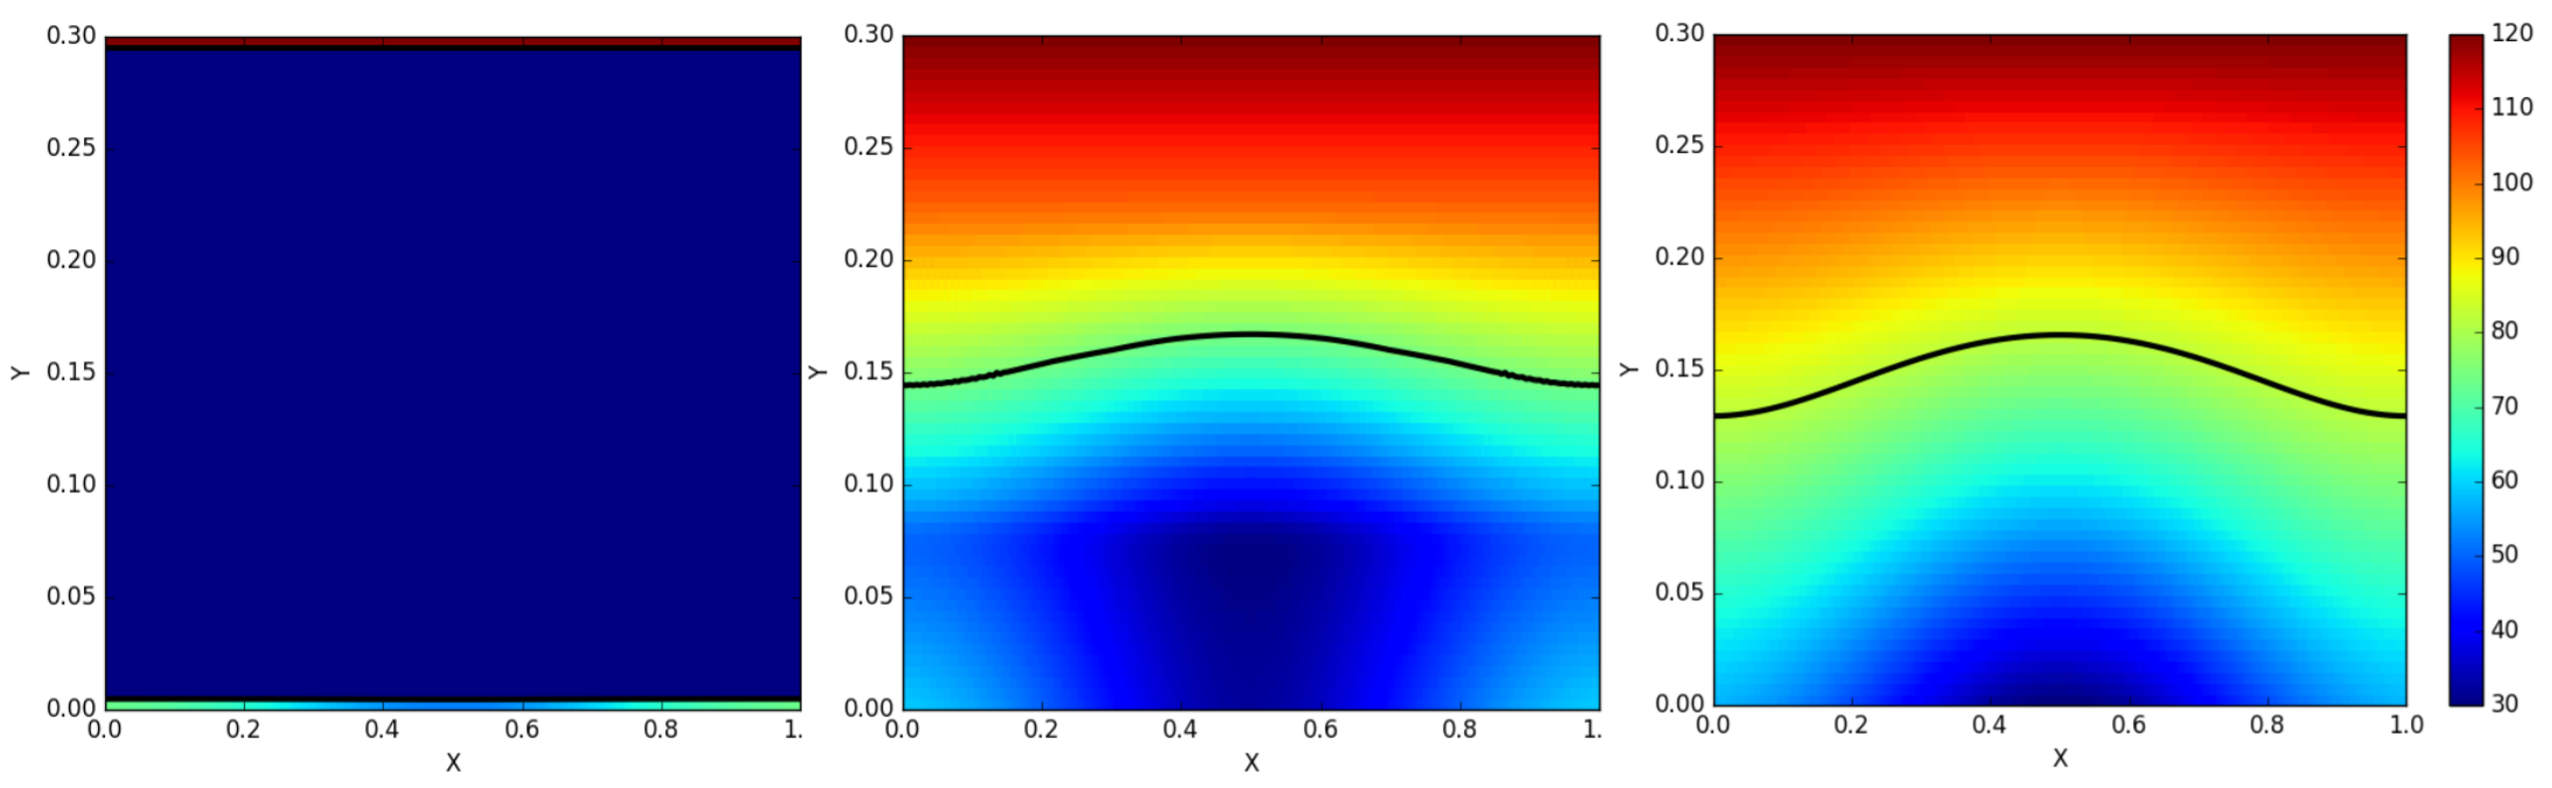
\includegraphics[width=1.1\textwidth]{visualization.png}
\caption{Solution iterates of the CG method from left to right: Initial guess, solution after 80 iterations, converged solution after 157 iterations. The black line is the isoline of the average temperature in the rod.}
\label{fig}
\end{figure}

\section{List of files}
\begin{enumerate}

\item \texttt{CGSolver.cpp, CGSolver.hpp} \citep{files2}

\item \texttt{COO2CSR.cpp, COO2CSR.hpp} \citep{files}

\item \texttt{heat.cpp, heat.hpp} \citep{files2}

\item \texttt{matvecops.cpp, matvecops.hpp}

\item \texttt{sparse.cpp, sparse.hpp} \citep{files2}

\item \texttt{main.cpp} \citep{files2}

\item \texttt{makefile}

\item \texttt{postprocess.py}

\item \texttt{input0.txt, input1.txt, input2.txt} \citep{files}
\end{enumerate}

\bibliography{project}

\end{document}
